\chapter{FUNDAMENTAÇÃO TEÓRICA}\label{cap:fundamentacao-teorica}


Neste capítulo são apresentados vários conceitos e técnicas para fundamentar
o desenvolvimento do método proposto, descrito na seção~\ref{sec:teorica-egsis}.


\section{Segmentação interativa de imagens}\label{sec:segmentacao-interativa}

A segmentação interativa de imagens é um processo de divisão de uma
imagem digital em várias partes ou regiões, geralmente para tornar a
imagem mais fácil de analisar e processar~\cite{ramadan2020survey}. Este processo é `interativo'
porque envolve a entrada do usuário para ajudar a orientar ou refinar
o processo de segmentação.

\begin{figure}[h!]
        \captionsetup{width=12cm}
		\Caption{\label{fig:interactive-segmentation}
          O usuário marca anotações do fundo e do objeto a ser
          segmentado, então a segmentação interativa é realizada.
        }
		\centering
		\UFCfig{}{\fbox{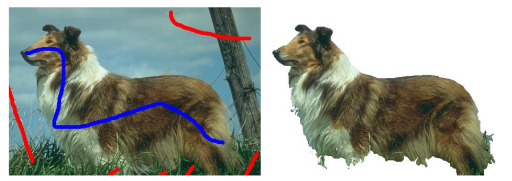
\includegraphics[width=12cm]{figuras/interactive-segmentation-2008}}}{\Fonte{\cite{duchenne2008segmentation}}}
\end{figure}
\FloatBarrier{}

De acordo com a figura~\ref{fig:interactive-segmentation}, na
segmentação interativa de imagens, o usuário pode selecionar regiões
de interesse, definir marcadores ou fazer anotações na imagem. Essas
entradas do usuário são então usadas para informar o algoritmo de
segmentação sobre como dividir a imagem. Por exemplo, o usuário pode
desenhar uma linha ao redor de um objeto de interesse, e o algoritmo
de segmentação irá então tentar dividir a imagem de tal forma que o
objeto de interesse seja isolado em sua própria região.

Este tipo de segmentação de imagem é útil em uma variedade de
aplicações, incluindo processamento de imagens médicas, visão
computacional, reconhecimento de padrões e muitos outros campos onde é
útil poder dividir uma imagem em regiões distintas com base em
critérios definidos pelo usuário.

\section{Aprendizado semi-supervisionado vs.\ transdução}\label{sec:teorica-aprendizado-semi-supervisionado}

Existem três principais categorias de aprendizado de máquina:
aprendizado supervisionado, aprendizado não-supervisionado e
aprendizado semi-supervisionado. No aprendizado supervisionado durante
a etapa de treinamento existe uma base de dados totalmente rotulada,
no aprendizado não-supervisionado não é disponibilizado nenhum
rotulamento dos dados. Enquanto isso, o aprendizado
semi-supervisionado está entre essas duas categorias.

O aprendizado semi-supervisionado é um método de aprendizado de máquina
que envolve o uso de um grande volume de dados não rotulados e um
pequeno volume de dados rotulados para treinar modelos de aprendizado
de máquina.

Formalmente, pode-se definir o aprendizado semi-supervisionado da seguinte maneira:

\begin{quote}
  Dado um conjunto de dados de treinamento
  $ \mathbf{X} = \{\vec{x_1}, \vec{x_2}, \ldots, \vec{x_n}\} $, tal que $ \vec{x_n} \in \mathbb{R}^d $,
  onde apenas um subconjunto  $ \vec{Y} = \{y_1, y_2, \ldots , y_m\} $ em que $ (m < n) $ tem rótulos
  correspondentes, o objetivo do aprendizado semi-supervisionado é usar
  tanto o conjunto de dados rotulado quanto o não rotulado para aprender
  a função $ f: \mathbf{X} \rightarrow \vec{Y} $ que pode prever o rótulo $ y $ para um novo
  exemplo $ \vec{x} $.
\end{quote}

O aprendizado semi-supervisionado é baseado na suposição de que os
dados não rotulados podem fornecer informações adicionais que podem
ser usadas para melhorar a precisão do modelo de aprendizado de
máquina. Isso é feito através de várias técnicas, como a propagação de
rótulos, na qual os rótulos são propagados dos dados rotulados para os
dados não rotulados, ou a aprendizagem auto-supervisionada, onde o
modelo é treinado para prever partes dos dados a partir de outras
partes.

Por outro lado, existe um diferente tipo de aprendizado
semi-supervisionado que não realiza a etapa de estimar a função $ f
$. Algoritmos que estimam essa função são descritos como indutivos,
pois após o treinamento, para classificar novos dados, realizam uma
inferência por indução ao aplicar a função estimada.

Em contraponto, existem algoritmos que não estimam tal função e apenas
realizam a inferência direta entre os dados rotulados disponíveis e os
não rotulados. Isso é chamado de transdução e um algoritmo bem
conhecido com essa característica é o classificador \gls{k-NN}.\@ Na
figura~\ref{fig:induction-vs-transduction} são ilustradas as
diferenças entre transdução e indução no processo de aprendizagem:


\begin{figure}[h!]
        \captionsetup{width=12cm}
		\Caption{\label{fig:induction-vs-transduction}
          No aprendizado transdutivo, a inferência em novos exemplos
          ocorre de maneira direta.
        }
		\centering
		\UFCfig{}{\fbox{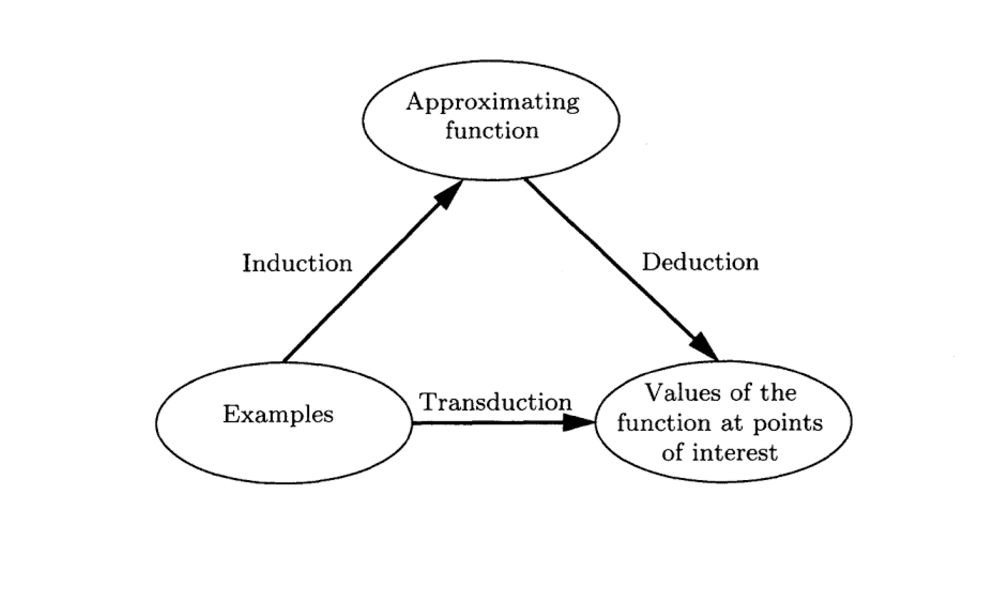
\includegraphics[width=12cm]{figuras/induction_vs_transduction}}}{\Fonte{\cite{vapnik1995}}}
\end{figure}


No texto~\cite{vapnik2006semi}, o criador do famoso algoritmo SVM,
estabelece uma profunda formalização dos problemas de aprendizado
semi-supervisionado e inferência transdutiva. No final do texto, ele declara
algumas reflexões sobre a solução de problemas em aprendizagem de
máquina. Em uma delas, ele diz que ao resolver um problema, não tente
resolver o problema geral como um passo intermediário, tente obter a
resposta que você precisa, mas não a mais geral. Por fim, Vapnik
deixa uma sugestão relevante:


\begin{displayquote}

  Do not estimate a function if you need to estimate values at given
  points. (Try to perform transduction, not induction.)

\end{displayquote}

Em tradução-livre: \blockquote{Não estime uma função se você precisa estimar
os valores em dados pontos. (Tente executar transdução, não
indução)}. Essa sugestão é uma evidência que reforça a motivação
deste trabalho. Ao desenvolver um algoritmo transdutivo pra
segmentação de imagens de maneira assistida, não é estimada uma função
geral como um passo intermediário, mas a segmentação é realizada
diretamente baseada nas rotulações iniciais que o usuário forneceu.


\section{Superpixels}\label{sec:teorica-superpixel}

Superpixels fazem parte de um grupo de algoritmos de clusterização em
processamento de imagens que ganhou popularidade nos últimos anos na
comunidade de visão computacional~\cite{SuperpixelSurvey2020}. Em vez
de processar uma imagem pixel por pixel, agrupam-se pixels vizinhos
semelhantes em uma entidade maior, conhecida como superpixel.

O conceito de superpixels foi introduzido para superar as limitações
do processamento pixel a pixel, que não leva em consideração a
estrutura global da imagem. Os superpixels, por outro lado, mantêm a
estrutura da imagem e reduzem a complexidade do processamento de
imagens, tornando-o mais eficiente.

Os superpixels são formados com base na similaridade dos pixels em
termos de cor, intensidade e localização na imagem. Eles são usados em
uma variedade de aplicações, incluindo segmentação de imagem,
rastreamento de objetos, reconhecimento de objetos, entre outros.

Em resumo, os superpixels são uma técnica eficaz para simplificar a
representação de uma imagem e aumentar a eficiência do processamento
de imagens, mantendo a informação visual importante.

Atualmente, já é possível encontrar muitas técnicas baseadas em
superpixels com diferentes características, complexidades
computacionais, métodos e eficiência. No
artigo~\cite{SuperPixelBenchmark2017}, é realizado um \textit{benchmark} com 15
algoritmos do tipo superpixel categorizados em três grupos: basedo em grafos,
baseado em otimização de gradiente e baseado em análise de
textura. Neste trabalho, é selecionado um dos mais simples: \gls{SLIC}.

\subsection{SLIC}\label{sec:teorica-superpixel-slic}


O algoritmo \gls{SLIC}~\cite{achanta2010slic} é um método para segmentação de imagens baseado
em superpixel, é um dos mais simples e pode ser visto como uma
variação do algoritmo de clusterização k-means expandindo o espaço
euclidiano ao incluir também o espaço de cores. Ele divide uma imagem
em segmentos menores, chamados superpixels, que compartilham
características semelhantes, como cor e textura.

Uma explicação passo-a-passo de como o SLIC funciona pode ser entendida
dessa maneira:

\begin{algorithm}[h!]
	\SetSpacedAlgorithm{}
	\caption{\label{alg:slic} SLIC}
	\Entrada{Imagem a ser segmentada}
    \Resultado{Matriz de superpixels}
	\Inicio{
      \begin{enumerate}

      \item \textbf{Inicialização}: O algoritmo começa selecionando alguns pixels na
        imagem como centros de superpixels. Esses centros são espaçados
        uniformemente pela imagem;

      \item \textbf{Atribuição}: Em seguida, para cada pixel na imagem, o algoritmo
        calcula a distância entre esse pixel e todos os centros de
        superpixels. A distância é calculada com base na cor (ou intensidade
        de níveis de cinza) e na proximidade espacial. O
        pixel é então atribuído ao superpixel cujo centro está mais próximo;

      \item \textbf{Atualização}: Depois que todos os pixels foram atribuídos a um
        superpixel, o algoritmo recalcula os centros de superpixels como a
        média de todos os pixels dentro de cada superpixel;

      \item O processo de atribuição e atualização é repetido várias vezes
        até que o algoritmo alcance a condição de convergência, ou seja, até
        que os centros de superpixels parem de mudar significativamente;

      \item O resultado final é uma segmentação da imagem em superpixels, onde
        cada superpixel é um grupo de pixels com características semelhantes.
    \end{enumerate}
   }
\end{algorithm}


Uma execução do SLIC é possível de ser visualizada a seguir:

\begin{figure}[h!]
        \captionsetup{width=12cm}
		\Caption{\label{fig:slic}
          Execução do algoritmo SLIC na fotografia de um gato.
        }
		\centering
		\UFCfig{}{\fbox{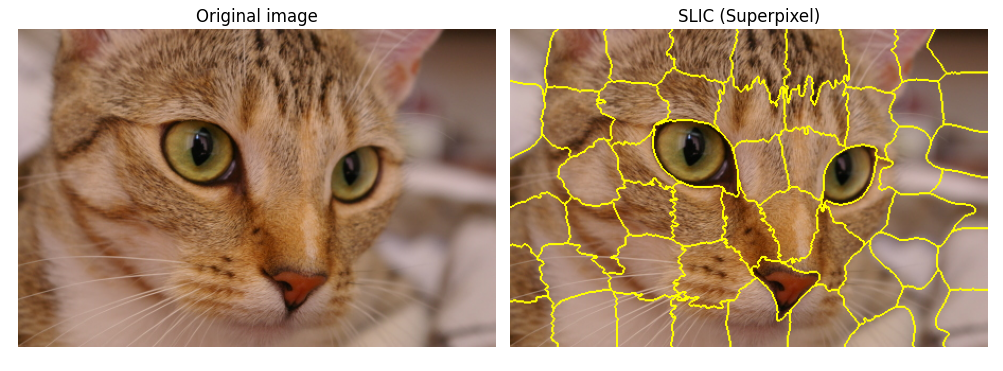
\includegraphics[width=12cm]{figuras/slic}}}{\Fonte{\fonteautor}}
\end{figure}

O algoritmo \gls{SLIC} possuí três hiperparâmetros: \textit{segments}, sigma e \textit{compactness}.

\begin{enumerate}
\item \textbf{Segments}: Número de superpixels que será usado para
  segmentar a imagem.
\item \textbf{Sigma}: Este parâmetro é usado para suavizar a imagem antes da
segmentação. Um valor maior de sigma resultará em uma imagem mais
suave, o que pode ajudar a reduzir o ruído e os detalhes finos. No
entanto, um valor muito alto pode resultar em perda de detalhes
importantes.
\item \textbf{Compactness} Este parâmetro controla o equilíbrio entre a coerência
de cor e a proximidade espacial na formação de superpixels. Um valor
maior de compactness fará com que os superpixels sejam mais
quadrados, enquanto um valor menor fará com que os superpixels
sigam mais de perto os limites da imagem. Portanto, a compactness pode
ser ajustada para obter superpixels que são mais representativos da
estrutura da imagem.
\end{enumerate}


\section{Geração de redes complexas}\label{sec:teorica-redes-complexas}

Redes complexas são grafos de alta complexidade. Existem variados
algoritmos para geração de redes complexas
~\cite{ComplexNetworksSurvey2007}. Redes complexas podem ser usadas
como um domínio de dados para realizar tarefas como classificação de
imagens~\cite{ComplexNetworksImageClassification2015}, segmentação de
imagens, identificação de comunidades e também extração de
características~\cite{JarbasComplexNetworks2020}.

Neste trabalho, o uso de redes complexas é realizado de uma maneira
acoplada ao algoritmo de clusterização inicial da imagem (superpixel). Nesse
cenário, cada superpixel gerado na imagem é um vértice e as arestas
são gerados com base na vizinhança.

Apesar de considerar o tema como redes complexas, esse cenário em
particular gera um grafo planar pela maneira como as arestas são
criadas. Por outro lado, seria possível também modificar a geração da
rede complexa para considerar as arestas do grafo baseado num raio
parametrizado de superpixel em relação a um \textit{treshrold} e
selecionar as \gls{k-NN} similares como arestas válidas.

Essa etapa de geração da rede complexa é crucial para a execução da
dinâmica coletiva explorada na seção~\ref{sec:teorica-lcu}, que é um dos
pontos centrais deste trabalho. Na figura~\ref{fig:complex-networks},
um exemplo de geração de rede complexa é apresentado conectado com a
ilustração~\ref{fig:slic}, ao executar o algoritmo SLIC.\@

\begin{figure}[t]
        \captionsetup{width=12cm}
		\Caption{\label{fig:complex-networks}
          Geração de rede complexa baseado nos superpixels.
        }
		\centering
		\UFCfig{}{\fbox{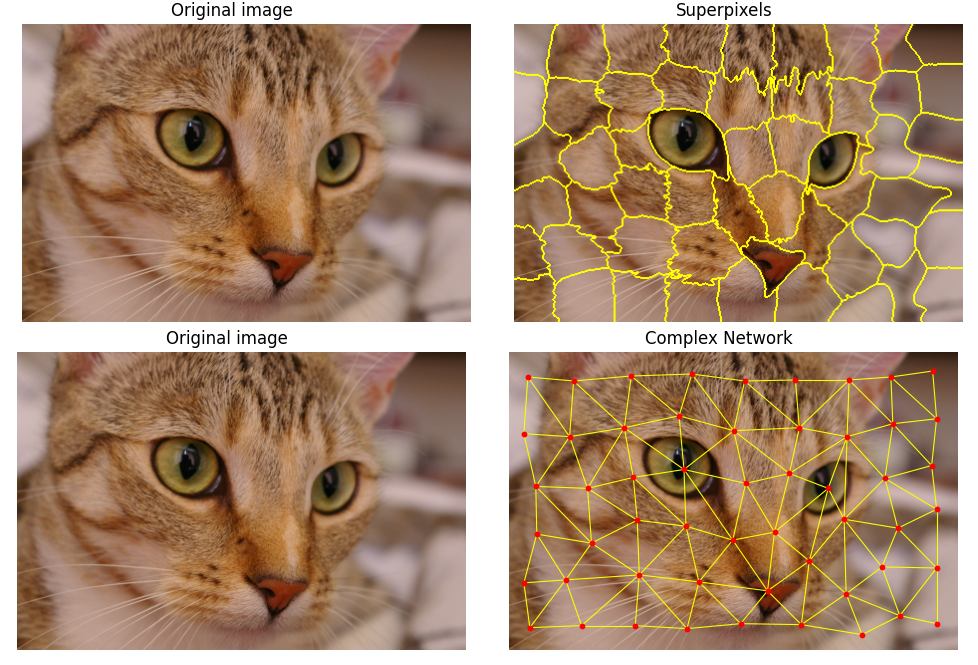
\includegraphics[width=12cm]{figuras/complex-networks}}}{\Fonte{\fonteautor}}
\end{figure}
\FloatBarrier{}

\section{Extração de características}\label{sec:extracao-caracteristicas}

\subsection{Matriz de co-ocorrências}\label{sec:teorica-matriz-co-ocorrencia}

O método de extração de características através de matriz de
co-ocorrências, originalmente proposto por Haralick em
\textit{\blockquote{Statistical and structural approaches to
texture}}~\cite{haralick1979statistical}, é uma técnica utilizada em
processamento de imagem e visão computacional para extrair
características texturais de uma imagem.

Formalmente, uma matriz de co-ocorrência $C$ é definida sobre uma imagem
$I$, para um deslocamento $\Delta x, \Delta y$, como:

\begin{equation}\label{eq:comatrix}
  C_{\Delta x, \Delta y}(i,j) = \sum_{x=1}^n\sum_{y=1}^m
  \begin{cases} 1, & \text{if }I(x,y)=i\text{ e }I(x+\Delta x, y+\Delta y)=j
               \\ 0, & \text{caso contrário}
  \end{cases}
\end{equation}

Na equação~\ref{eq:comatrix} $C_{\Delta x, \Delta y}(i,j)$ é o número de vezes
que o par de pixels com intensidades $i$ e $j$ ocorre em dois pixels
separados pelas distâncias (horizontal e vertical) na imagem $I$.

A matriz de co-ocorrência é tipicamente normalizada dividindo cada
elemento pelo número total de pares de pixels na imagem, resultando em
uma matriz de probabilidade de co-ocorrência.

A partir desta matriz, várias características texturais podem ser
extraídas, como contraste, correlação, energia e homogeneidade. Estas
características podem ser usadas para tarefas como classificação de
textura, segmentação de imagem, entre outros. Após a aplicação do
método em cada canal RGB da imagem, são extraídas cinco estatísticas: média,
mediana, variância, desvio padrão e 25-quantis. Então as
características são concatenadas um vetor de características de 15 dimensões.

\subsection{Filtros de Gabor}\label{sec:filtros-gabor}

Os filtros de Gabor, originalmente proposto por Daugman em
\textit{\blockquote{Complete discrete 2-D Gabor transforms by neural
networks for image analysis and
compression}}~\cite{daugman1988complete}, são uma família de filtros
de convolução usados principalmente na análise de texturas e na visão
computacional para a extração de características. Eles são nomeados em
homenagem a Dennis Gabor, o físico que ganhou o Prêmio Nobel por sua
invenção e desenvolvimento do método holográfico.

Os filtros de Gabor são essencialmente filtros passa-banda orientados
e localizados no espaço de frequência. Eles são muito úteis para a
extração de características porque têm propriedades ótimas de
localização no espaço e na frequência, o que os torna muito adequados
para a captura de características locais e direcionais em uma imagem.

Os filtros de Gabor são definidos por duas funções: uma função
gaussiana (para o domínio espacial) e uma função harmônica complexa
(para o domínio da frequência). A função gaussiana serve para limitar
a aplicação do filtro a uma pequena região da imagem (localização
espacial), enquanto a função harmônica complexa permite capturar
características em uma determinada orientação. Na
figura~\ref{fig:gabor-filters} são ilustrados variações dos
filtros de Gabor com diferentes parâmetros e a convolução resultante.

\begin{figure}[!h]
        \captionsetup{width=12cm}
		\Caption{\label{fig:gabor-filters}
          Filtros de Gabor variando a angulação $\theta$ e a convolução resultante.
        }
		\centering
		\UFCfig{}{\fbox{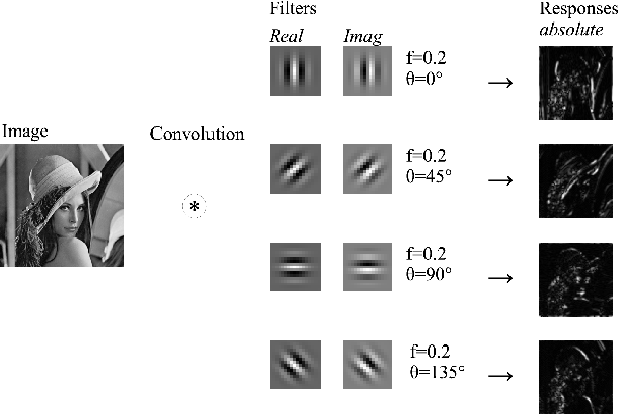
\includegraphics[width=12cm]{figuras/gabor-filters}}}{\Fonte{\cite{Kmrinen2012GaborFI}}}
\end{figure}
\FloatBarrier{}

A operação de convolução entre uma imagem qualquer $ x $ e um filtro de
Gabor $ k $, pode ser dada pela seguinte equação:

\begin{equation}
  (y * k)(i, j) = \sum_{m} \sum_{n} x(i-m, j-n) k(m, n)
\end{equation}

A extração de características usando filtros de Gabor geralmente
envolve a convolução da imagem com um conjunto de filtros de
Gabor. Cada filtro é sensível a características de uma determinada
escala e orientação. A resposta do filtro pode então ser usada como
uma representação da presença de tais características na imagem.

Neste trabalho, são gerados 16 filtros de Gabor que foram avaliados
experimentalmente com variados parâmetros. Após a aplicação do filtro
em cada canal RGB da imagem, são extraídos cinco estatísticas: média,
mediana, variância, desvio padrão e 25-quantis. Com isso, todas as
estatisticas são concatenadas num único vetor de características
resultante com 63 dimensões.

\section{Métricas de similaridade}\label{sec:teorica-metricas-de-similaridade}


Métricas de similaridade neste trabalho são calculadas com o propósito
de comparar a similaridade entre os vetores de características dos
superpixels. Para as técnicas de extração de características descritas
na seção~\ref{sec:extracao-caracteristicas}, cada técnica se comportou
melhor com uma métrica de similaridade diferente.

Uma função de similaridade entre dois vetores de características
retorna um valor maior quando os vetores são similares e quanto mais
diferentes sejam, mais a similaridade tende a zero.

A estrutura de uma métrica de similaridade pode ser criada a partir de
uma métrica de distância. Neste trabalho, são exploradas duas métricas de
similaridades a partir das seguintes métricas de distância: distância
euclidiana e distância de manhattan.

A distância euclidiana é o módulo da reta que conecta dois pontos no
espaço. A distância de manhattan é a soma da diferença absoluta entre
dois pontos para cada dimensão. Na
figura~\ref{fig:manhattan-vs-euclidean} é ilustrado a disposição de
dois pontos $ x $ e $ y $ no espaço euclidiano com os módulos de
segmento de reta usados para compor a distância de cada métrica.

\begin{figure}[!h]
        \captionsetup{width=8cm}
		\Caption{\label{fig:manhattan-vs-euclidean}
          Visualização da distância de manhattan e distância euclidiana.
        }
		\centering
		\UFCfig{}{\fbox{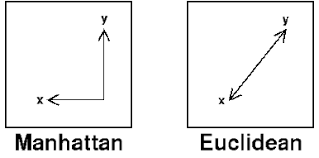
\includegraphics[width=8cm]{figuras/manhattan-vs-euclidean}}}{\Fonte{\cite{Singh2019}}}
\end{figure}
\FloatBarrier{}

Para as equações das distâncias, tem-se a seguinte equação para a
distância euclidiana:

\begin{equation}\label{eq:euclidian-distance}
ed(\vec{x}, \vec{y}) = \sqrt{{(y_1-x_1)}^2 + {(y_2-x_2)}^2 + \cdots + {(y_n-x_n)}^2}
\end{equation}

Para a distância de manhattan, tem-se a seguinte equação:

\begin{equation}\label{eq:manhattan-distance}
md(\vec{x}, \vec{y}) = |y_1-x_1| + |y_2-x_2| + \cdots + |y_n-x_n|
\end{equation}

\subsection{Similaridade Euclidiana Exponencial}\label{sec:teorica-similaridade-euclidiana}

Para a técnica de extração de característica de matrizes de co-ocorrência,
detalhada na seção~\ref{sec:teorica-matriz-co-ocorrencia}, a métrica de
similaridade que obteve os melhores resultados foi a distância
euclidiana pelo inverso da exponencial. A equação é definida como:

\begin{equation}\label{eq:euclidian-similarity}
  ed\_sim(\vec{x}, \vec{y}) = \dfrac{1}{e^{ed(\vec{x}, \vec{y})}}
\end{equation}

\subsection{Similaridade de Manhattan Logarítmica}\label{sec:teorica-similaridade-manhattan}

Para a técnica envolvendo filtros de Gabor, a distância entre os
vetores de características tiveram valores tão altos que ao usar a
similaridade euclidiana (exponencial ou não), maior parte dos valores
chegavam a zero. Por esse motivo, o uso da conversão para o domínio
logarítmico foi usado para suavizar o crescimento exagerado dos
valores, obtendo bons resultados. A definição para essa equação de
similaridade segue a seguir:

\begin{equation}\label{eq:manhattan-similarity}
  md\_sim(\vec{x}, \vec{y}) = \dfrac{1}{1 + \ln(1 + md(\vec{x}, \vec{y}))}
\end{equation}

Na equação~\ref{eq:manhattan-similarity}, os valores $1$ adicionados
ao demoninador foram necessários para evitar uma possível divisão por
zero e logarítmo de zero, ambas operações que são indefinidas na
matemática.


\section{LCU}\label{sec:teorica-lcu}

O algoritmo \gls{LCU} foi desenvolvido por um
brasileiro~\cite{VerriNetworkUnfoldingMap2018}, é uma dinâmica
coletiva baseada em propagação de rótulos numa rede complexa. Essa
dinâmica coletiva é modelada como um sistema dinâmico com geração de
partículas de rotulação nas suas fontes (os vértices rotulados).

Esse algoritmo possui critérios de sobrevivência das particulas
inspirado em comportamentos da natureza e sociedade. Por exemplo, o
hiperparâmetro $ \lambda $ do algoritmo denota um fator de competição entre
0 e 1 sobre o dificuldade que as partículas terão ao trafegar nos
vértices, tornando a sobrevivência delas mais difícil ao percorrer o
grafo. Para esse parâmetro, 0 significa um passeio aleatório no grafo,
1 significa máxima competitividade. Embora as partículas nasçam nos
vértices, a competição por dominação acontece nas arestas. No final, o
vértice será marcado com o novo rótulo baseado no tipo de partícula
que mais conseguiu dominar arestas desse vértice.

Nesse caso particular, a implementação proposta neste trabalho é
ligeiramente diferente da proposta originalmente, pois a rede complexa
no cenário que o autor propõe as arestas não possuem peso. Uma
modificação é realizada para incluir a similaridade de imagem entre
dois superpixels, dessa maneira é criado um fator de aumento da
probabilidade das partículas visitarem os nós mais promissores
(texturas mais similares). Como discutido na
seção~\ref{sec:teorica-aprendizado-semi-supervisionado}, esse cenário
de aprendizado é semi-supervisionado transdutivo: poucos rótulos estão
disponíveis e nenhuma função de inferência é estimada. A inferência
acontece diretamente entre os pontos rotulados e os não-rotulados.


\begin{figure}[!h]
\centering
    \captionsetup{width=14cm}
    \Caption{\label{fig:lcu-execution}
      Rede complexa para execução da dinâmica LCU.\@ Anotação
      parcial em~(\subref{fig:lcu-partial}) e resultado final em~(\subref{fig:lcu-done})
    }

    \begin{subfigure}[b]{0.45\textwidth}
    \centering
    \UFCfig{}{\fbox{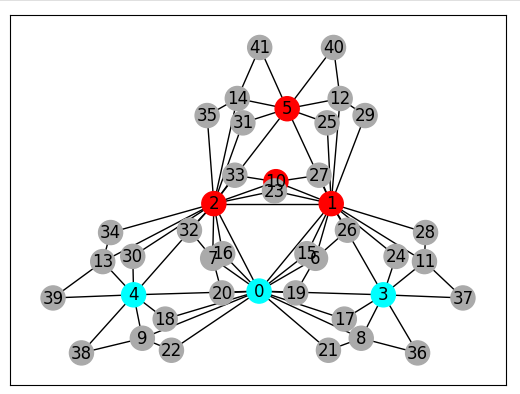
\includegraphics[width=7cm]{figuras/lcu-partial}}}
    \caption{\label{fig:lcu-partial}}
    \end{subfigure}
\quad
    \begin{subfigure}[b]{0.45\textwidth}
    \centering
    \UFCfig{}{\fbox{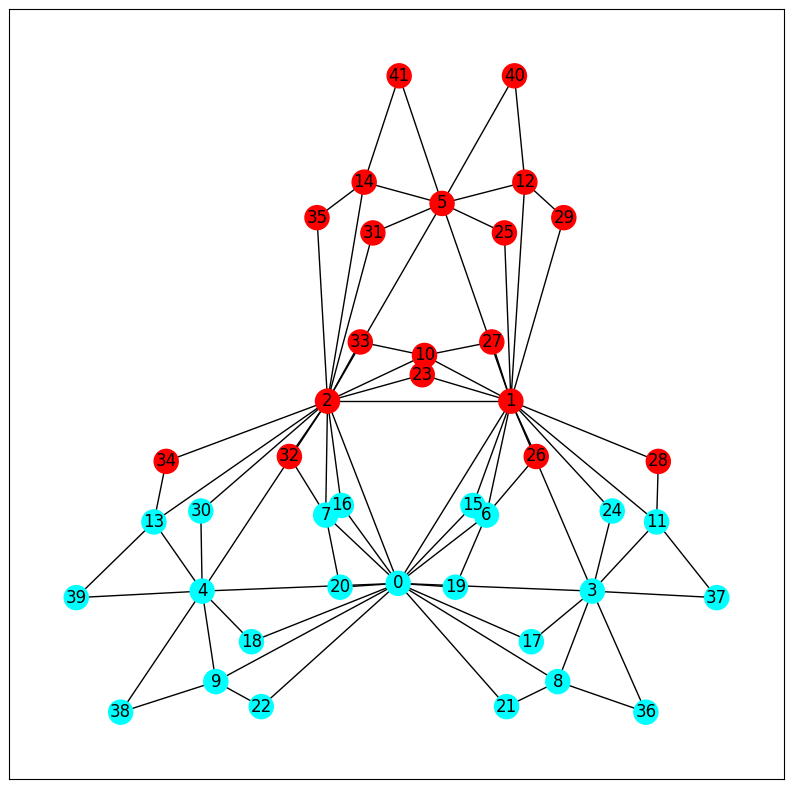
\includegraphics[width=7cm]{figuras/lcu-done}}}
    \caption{\label{fig:lcu-done}}
    \end{subfigure}
    {\Fonte{\fonteautor}}
\quad
\end{figure}
\FloatBarrier{}


Na figura~\ref{fig:lcu-execution}, é possível ver a execução do
algoritmo numa rede complexa densa aleatória, no início há alguns
poucos vértices anotados em azul e vermelho. No final da execução os
rótulos são propagados semanticamente baseado na disputa entre as
partículas para dominar arestas, e por fim, marcar os vértices
dominados por aquela classe.

Em mais detalhes, durante uma única iteração do sistema na
figura~\ref{fig:lcu-iteration}, pode-se visualizar o passeio das
partículas entre as fontes de párticulas (vértices rotulados) verde e
vermelho. Algumas não sobreviveram ao processo, outras se mantiveram
no sistema. Na última imagem, uma contagem do número de partículas por
classe que passaram pelas arestas pode ser vista.


\begin{figure}[h!]
        \captionsetup{width=8cm}
		\Caption{\label{fig:lcu-iteration}
          Iteração do sistema LCU em um grafo planar.
        }
		\centering
		\UFCfig{}{\fbox{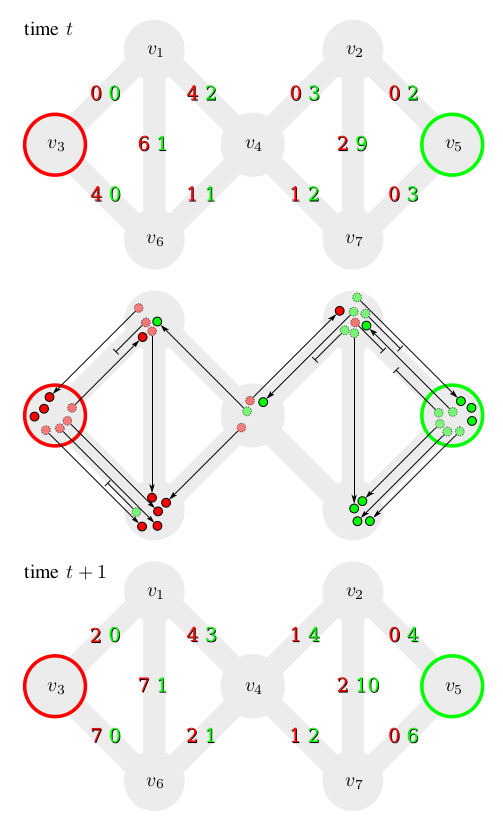
\includegraphics[width=8cm]{figuras/lcu-iteration}}}{\Fonte{\cite{VerriNetworkUnfoldingMap2018}}}
\end{figure}


\subsection{Modelagem matemática LCU com grafo ponderado}\label{sec:lcu-math}

Considera-se uma rede complexa expressada por um simples grafo
ponderado não-direcionado $G = (\mathcal{V}, \mathcal{E})$, onde $\mathcal{V}$ é o conjunto de
vértices e $\mathcal{E} \subset \mathcal{V} \times \mathcal{V}$ é o conjunto de arestas. A rede possui
$\left|\mathcal{V}\right| = l + u$ vértices que podem ser representações de
dados rotulados ($ l $) ou não-rotulados ($ u $). Os vértices anotados
podem ter um rótulo $y_i = \{1, \ldots, C\}$, em que $C$ é o número total de
classes, além disso possuem um vetor de características $\vec{x_i}$ da
representação daquele dado. A rede é representada por uma matriz de
adjacência $A = (a_{ij})$, onde $a_{ij} =a_{ji} =
similarity(\vec{x_i}, \vec{x_j})$, na qual as arestas possuem um peso
que se refere à similaridade entre os vetores de características
representados pelos vértices. Nessa situação, supõe-se que $l << u$,
ou seja, há muito mais dados não-rotulados do que rotulados, na qual
caracteriza-se um cenário para aprendizado semi-supervisioado.

Os vértices rotulados são chamados de fontes, que geram partículas com
a classe que responde ao vértice. Partículas que alcançam um vértice fonte
com classe diferente são eliminados automaticamente do sistema.

O sistema dinâmico não-linear $X(t)$ que representa o \gls{LCU} é definido
matematicamente como:

\begin{equation}\label{eq:lcu-x}
  X(t):=\left[\begin{array}{c}
    \mathbf{n}^c(t)={\left[n_i^c(t)\right]}_i \\
    N^c(t)={\left(n_{i j}^c(t)\right)}_{i, j} \\
    \Delta^c(t)={\left(\delta_{i j}^c(t)\right)}_{i, j}
\end{array}\right]
\end{equation}

\noindent
Em que $ \mathbf{n}^c(t)$ é um vetor linha cujo elementos $n_i^c(t)$
representam a população de partículas com rótulo $c$ em cada vértice
$v_i$ no tempo $t$. Os elementos $n_{i j}^c(t)$ representam o número
de partículas da classe $c$ que se movem do vértice $v_i$ para $v_j$ no
tempo $ t $, enquanto $\delta_{i j}^c(t)$ representa a movimentação
acumulada de partículas da classe $c$ entre a aresta $(i, j)$ no tempo
$t$.

A função determinística de evolução do sistema dinâmico é definida
por:

\begin{equation}\label{eq:lcu-phi-evolution}
  \phi:\left\{\begin{array}{l}
    \mathbf{n}^c(t+1)= P^c(X(t)) \times \mathbf{n}^c(t) +\mathbf{g}^c(X(t)) \\
    N^c(t+1)=\operatorname{diag} \mathbf{n}^c(t) \times P^c(X(t)) \\
    \Delta^c(t+1)=\Delta^c(t)+N^c(t+1),
  \end{array}\right.
\end{equation}

Entre as funções ainda não definidas na função de evolução, destaca-se a de
probabilidade de sobrevivência das partículas $P^c(X(t))$, na qual os
elementos dessa matriz são definidos como:

\begin{equation} \label{eq:lcu-probability}
  p_{i j}^c(X(t)):= \begin{cases}0 & \text { se } v_j \in \mathcal{L} \text { e
                                     } y_j \neq c, \\
    \frac{a_{i j}}{\deg v_i}\left(1-\lambda \sigma_{i
    j}^c(X(t))\right) & \text { do contrário }\end{cases}
\end{equation}
\noindent
Em que ${\deg v_i}$ o grau do vértice (número de arestas
conectadas) e variável $\sigma_{i j}^c$ define-se como:

\begin{equation}\label{eq:lcu-sigma}
\begin{aligned}
\sigma_{i j}^c(X(t)):= \begin{cases}1-\frac{n_{i j}^c(t)+n_{j i}^c(t)}{S} & \text { se } S>0, \\
1-\frac{1}{C} & \text { do contrário, }\end{cases} \\
\text { sendo } S=\sum_{q=1}^C n_{i j}^q(t)+n_{j i}^q(t) .
\end{aligned}
\end{equation}

A modificação dessa dinâmica coletiva em relação à proposta original
em~\cite{VerriNetworkUnfoldingMap2018} é realizada em $a_{ij}$,
enquanto no trabalho original o grafo é não-ponderado e, portanto,
todas as arestas possuem valor unitário. Neste trabalho a aresta representa um
valor de similaridade entre os vetores de características anexados ao
vértice $v_i$ e $v_j$, dessa maneira aumentando a probabilidade de
sobrevivência de partículas que se movimentam por arestas com maior
similaridade.

A última função $\mathbf{g}^c(X(t))$ representa a geração de
partículas nos vértices fontes no tempo $t$, e é definida como:

\begin{equation}\label{eq:lcu-generation}
  \begin{aligned}
    g_i^c(X(t)) &:=\rho_i^c \max \left\{0, \lVert \mathbf{n}^c(0) \rVert - \lVert \mathbf{n}^c(t) \rVert\right\} \\
    \rho_i^c &:= \begin{cases}\frac{\deg v_i}{\sum_{v_j \in \mathcal{G}^c}
      \deg v_j} & \text { se } v_i \in \mathcal{G}^c, \\ 0 & \text {
                                                               do contrário }\end{cases}
  \end{aligned}
\end{equation}

Na equação~\ref{eq:lcu-generation}, $\mathcal{G}^c = \{v_i |v_i \in \mathcal{L}, y_i = c\}$
é o conjunto de fontes de partículas que pertencem à classe $c$ e $\mathcal{L}$
é o conjunto dos vértices rotulados.


Após alcançar a iteração máxima de um valor escolhido para $ \tau $, é possível
dividir a rede complexa em sub-grafos, primeiramente agrupando as
arestas por maior dominação de classe:

\begin{equation}\label{eq:lcu-edges-by-class}
  \mathcal{E}^c(t):=\left\{(i, j) \mid \underset{q}{\arg \max }\left(\delta_{i j}^q(t)+\delta_{j i}^q(t)\right)=c\right\}
\end{equation}

E, então, define-se o grafo por classe $c$ como:

\begin{equation}\label{eq:lcu-subnetworks}
  G^c(t):=\left(\mathcal{V}, \mathcal{E}^c(t)\right)
\end{equation}

Por fim, as redes $ G^c(\tau) $ são usadas para classificação dos
vértices. São atribuídos os rótulos $y_j \in \{1, \ldots, C\}$ para cada
vértice não-rotulado com a informação provida pela rede $G^c$.  O
rótulo $y_j$ é atribuido baseado na densidade das arestas na sua
vizinhaça. Formalmente, escrito como:

\begin{equation}\label{eq:lcu-vertex-classification}
y_j = \underset{c \in \{1, \ldots, C\}}{\arg \max }\left| \mathcal{E}(\mathcal{N}_{c,j}) \right|
\end{equation}
\noindent
Em que ${\mathcal{N}_{c,j}}$ são as arestas da vizinhança do vértice $j$ que
foram dominadas por párticulas da classe $c$. Na
figura~\ref{fig:lcu-classification}, é ilustrada a dinâmica coletiva
aplicada em uma rede complexa de formato similar a duas bananas. A
ilustração está dividida em quatro etapas: (a) inicialização com 6
vértices rotulados, 3 para cada classe, vértices pretos não estão
rotulados; (b) 4 iterações do sistema, com as arestas coloridas
sendo dominadas por particulas, enquanto as cinzas ainda não foram
dominadas; (c) 20 iterações, todo o grafo foi percorrido; (d) a
classificação dos vértices pela classe correspondente que obteve maior
dominação.

\begin{figure}[h!]
        \captionsetup{width=12cm}
		\Caption{\label{fig:lcu-classification}
          Execução em quatro fases da dinâmica coletiva LCU.\@
        }
		\centering
		\UFCfig{}{\fbox{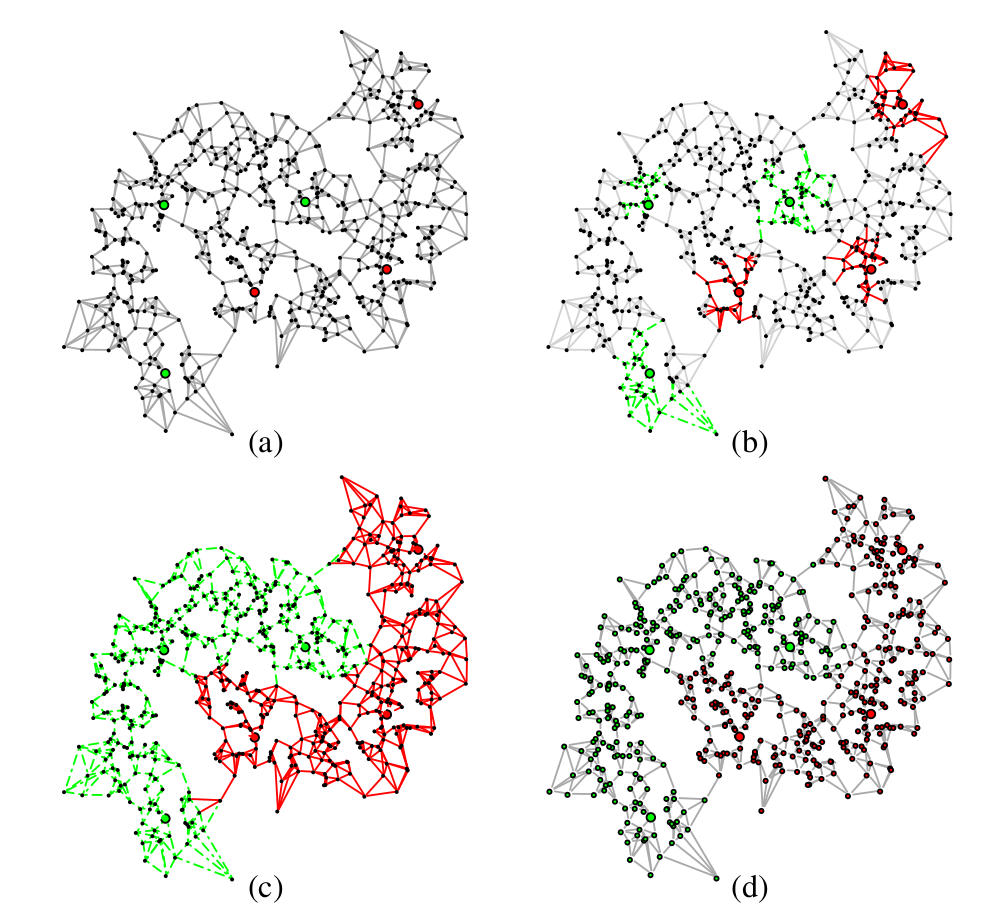
\includegraphics[width=12cm]{figuras/lcu-classification}}}{\Fonte{\cite{VerriNetworkUnfoldingMap2018}}}
\end{figure}

\section{EGSIS}\label{sec:teorica-egsis}

O algoritmo \gls{EGSIS} é a técnica de segmentação de imagens proposta
proposta neste trabalho. Todas as seções anteriores da fundamentação
teórica foram introduzidas para explicar o funcionamento dessa técnica
que será descrita nesta seção.

O modelo \gls{EGSIS} permite a execução de uma segmentação transdutiva
de imagens na presença de uma rotulação parcial da imagem. Essa
técnica possui etapas flexíveis para refinamento e otimização, quanto
a método de extração de características, quantidade de superpixels,
função de similaridade, entre outros.

Ao considerar as características do algoritmo LCU explicada na
seção~\ref{sec:teorica-lcu}, esse algoritmo também pode ser usado para
aprendizado semi-supervisionado multi-classe.

O ponto central desse método de segmentação é realizar uma
transformação do domínio da imagem para uma rede complexa que seja
compatível com a dinâmica coletiva \gls{LCU}. Para isso, uma
pré-segmentação é realizada usando superpixels através do algoritmo
SLIC.\@ Os rótulos iniciais da imagem são propagados aos superpixels
baseado numa votação: a classe que tiver maior números de pixels
rotulados, atribui-se aquela classe ao superpixel.

Ao obter os superpixels e os rótulos iniciais, é construída uma rede
complexa onde os vértices representam os superpixels e as arestas a
vizinhança com grau de similaridade entre os superpixels. Para
calcular a similaridade de cada aresta, primeiro é executado para cada
superpixel o metódo de extração de características selecionado, que
nesse caso pode ser filtros de Gabor ou matrizes de co-ocorrência,
então calcula-se a similaridade entre os superpixels com uma métrica
de similaridade selecionada.

Nessa etapa, a rede complexa é preparada para execução do sistema
dinâmico \gls{LCU} a fim de propagar os rótulos no grafo. No final da
execução do \gls{LCU}, é reconstruída uma máscara de segmentação
baseado nas rotulações dos vértices restantes em cada superpixel
não-rotulado. Por fim, obtém-se uma matriz de labels relacionando
cada pixel ao rótulo de segmentação desejado.

No Algoritmo~\ref{alg:egsis} são descritos as etapas do funcionamento
geral do método.

\begin{algorithm}[h!]
	\SetSpacedAlgorithm{}
	\caption{\label{alg:egsis} EGSIS}
	\Entrada{Imagem, rotulações parciais}
    \Resultado{Imagem segmentada}
	\Inicio{
      Inicializa os hiperparâmetros do modelo \gls{EGSIS}\;
      Segmenta a imagem em $n$ superpixels usando \gls{SLIC}\;
      Realiza a construção da rede complexa baseado nos superpixels\;
      Atribui os superpixels rotulados baseado na anotação parcial\;
      Calcula o vetor de características para cada superpixel\;
      Calcula a similaridade entre superpixels da vizinhança\;
      Executa a dinâmica LCU sobre a rede complexa gerada\;
      Reconstrói a máscara de segmentação com base nos vértices rotulados\;
   }
\end{algorithm}
\FloatBarrier

A seguir uma ilustração da execução do algoritmo em algumas etapas. Na
figura~\ref{fig:egsis-init}, são observadas duas etapas sendo
realizadas: na imagem (\subref{fig:egsis-superpixels}) a segmentação
por superpixels, na imagem (\subref{fig:egsis-complex-networks}) a rede
complexa gerada através dos superpixels.


\begin{figure}[!h]
\centering
    \captionsetup{width=14cm}
    \Caption{\label{fig:egsis-init}
      Construção de superpixels e a rede complexa no modelo EGSIS.\@
    }

    \begin{subfigure}[b]{0.45\textwidth}
    \centering
    \UFCfig{}{\fbox{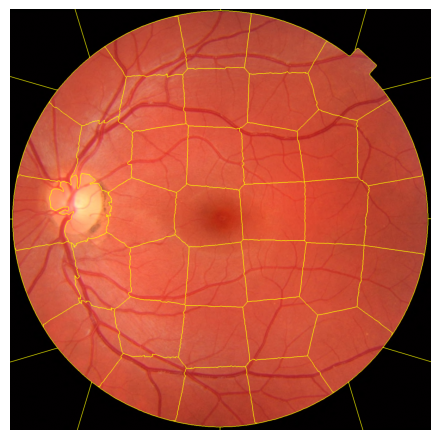
\includegraphics[width=7cm]{figuras/egsis-superpixels}}}
    \caption{\label{fig:egsis-superpixels}}
    \end{subfigure}
\quad
    \begin{subfigure}[b]{0.45\textwidth}
    \centering
    \UFCfig{}{\fbox{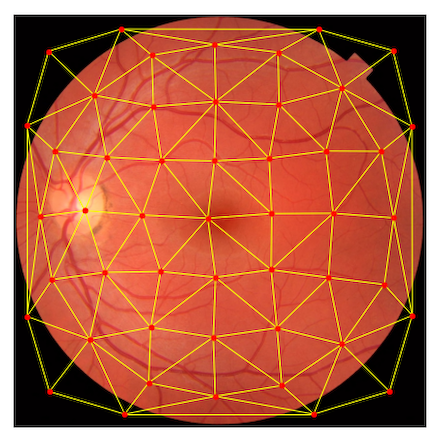
\includegraphics[width=7cm]{figuras/egsis-complex-networks}}}
    \caption{\label{fig:egsis-complex-networks}}
    \end{subfigure}
    {\Fonte{\fonteautor}}
\quad
\end{figure}
\FloatBarrier{}



Na figura~\ref{fig:egsis-lcu}, há alguns superpixels
anotados em azul e vermelho, e uma segmentação em duas classes. Na outra
imagem, é ilustrado o resultado após a continuação da
execução. Perceba que boa parte da imagem foi segmentada corretamente, mas houve
alguns erros visíveis.

\begin{figure}[!h]
\centering
    \captionsetup{width=14cm}
    \Caption{\label{fig:egsis-lcu}
      Etapa do método EGSIS para propagar rótulos iniciais através do
      sistema dinâmico LCU.\@
    }

    \begin{subfigure}[b]{0.45\textwidth}
    \centering
    \UFCfig{}{\fbox{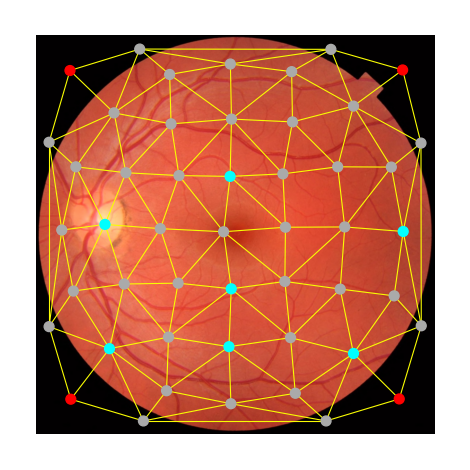
\includegraphics[width=7cm]{figuras/egsis-partial-labeled}}}
    \caption{\label{fig:egsis-partial-labeled}}
    \end{subfigure}
\quad
    \begin{subfigure}[b]{0.45\textwidth}
    \centering
    \UFCfig{}{\fbox{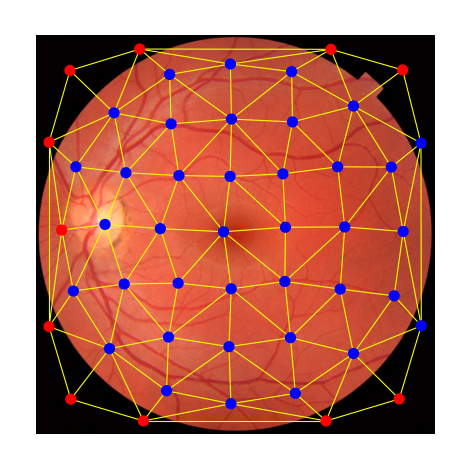
\includegraphics[width=7cm]{figuras/egsis-execution}}}
    \caption{\label{fig:egsis-execution}}
    \end{subfigure}
    {\Fonte{\fonteautor}}
\quad
\end{figure}
\FloatBarrier{}

Por fim, obtém-se a seguinte máscara de segmentação ao atribuir os
rótulos dos vértices para os superpixels iniciais, assim sendo
possível reconstruir uma máscara de segmentação como ilustrado na
figura~\ref{fig:egsis-mask}.

\begin{figure}[h!]
        \captionsetup{width=12cm}
		\Caption{\label{fig:egsis-mask}
          Máscara de segmentação final e a imagem original.\@
        }
		\centering
		\UFCfig{}{\fbox{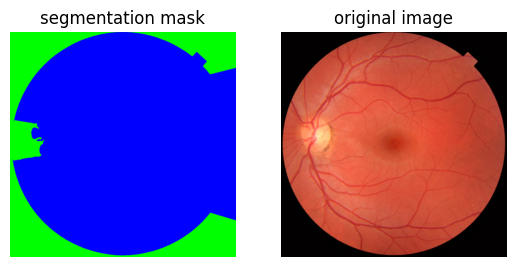
\includegraphics[width=12cm]{figuras/egsis-segmentation-mask}}}{\Fonte{\fonteautor}}
\end{figure}
